%%%%%%%%%%     BEAMER TEMPLATE     %%%%%%%%%%
%%%%%%%%%%       by Mason Reasner        %%%%%%%%%%

%%%	Setup	
%Basic
\documentclass[pslatex , slidestop, compress, table]{beamer}
\usepackage[utf8]{inputenc}

%Tikz
\usepackage{tikz, booktabs}
\usetikzlibrary{decorations.pathreplacing}
\usetikzlibrary{patterns}

%Theme and Colors
	%Base theme
	\usetheme{Madrid}
	
	%Set colors
	\definecolor{purduegold}{HTML}{CFB991}
	\definecolor{darkgray}{HTML}{333333}
	\definecolor{steel}{HTML}{555960}
	\definecolor{black}{HTML}{000000}
	\definecolor{lightgray}{HTML}{DDDDDD}
	
	%Frame title 
	\setbeamertemplate{frametitle}
	{
  		\nointerlineskip
   		\begin{beamercolorbox}[sep=0.3cm,ht=1.8em,wd=\paperwidth]{frametitle}
       			\vbox{}\vskip-2ex%
        			\strut\insertframetitle\strut
			%\hfill
			%\raisebox{-2mm}{\includegraphics[width=2cm]{logo.png}}
        			\vskip-0.7ex%
   		\end{beamercolorbox}
        		\nointerlineskip
		\begin{beamercolorbox}[wd=\paperwidth,ht=0.25em,center]{accent in head/foot}	
		\end{beamercolorbox}%
	}
	\setbeamercolor*{frametitle}{fg=white,bg=darkgray}
	\setbeamercolor*{accent in head/foot}{fg=white,bg=purduegold}
		
	%Footer
	\setbeamercolor*{author in head/foot}{bg=purduegold}
	\setbeamercolor*{title in head/foot}{bg=purduegold}
	\setbeamercolor*{date in head/foot}{bg=purduegold}
	
	%Title
	\setbeamercolor*{title}{fg=white,bg=purduegold}
	\titlegraphic{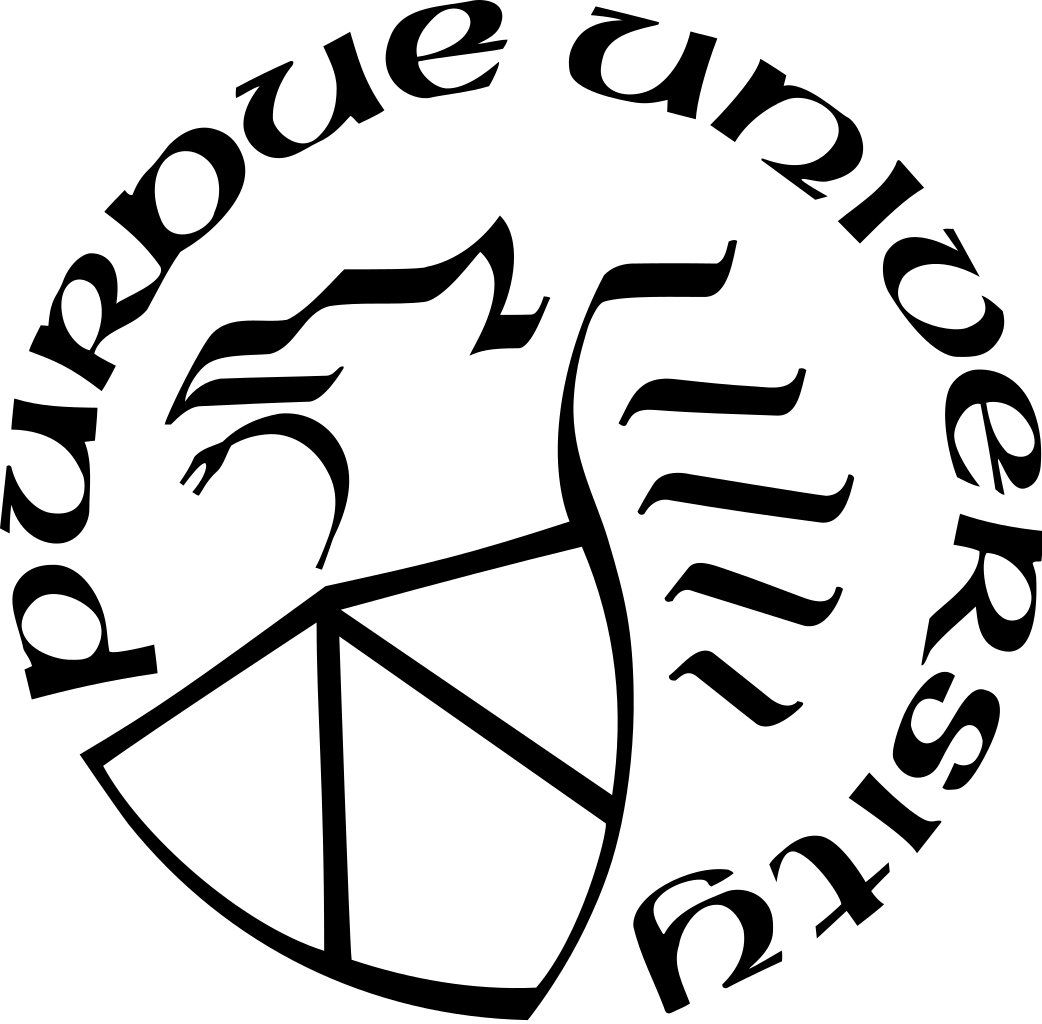
\includegraphics[height=.25\textheight]{seal.png}}
	\setbeamerfont{title}{size=\Huge}
	\setbeamerfont{author}{series=\bfseries,size=\large}
	\setbeamercolor*{author}{fg=black}
	\setbeamerfont{date}{size=\footnotesize}
	\setbeamercolor*{date}{fg=black}
	\setbeamercolor*{institute}{fg=black}

	%Fonts
	\setbeamercolor{normal text}{fg=steel}
	\usepackage{helvet}
	\usefonttheme[]{structurebold}	
	
	%Itemize
	\setbeamertemplate{itemize items}[circle]
	\setbeamercolor*{itemize item}{fg=purduegold}
	\setbeamertemplate{itemize subitems}[circle]
	\setbeamercolor*{itemize subitem}{fg=purduegold}
	\setbeamertemplate{itemize subsubitems}[circle]
	\setbeamercolor*{itemize subsubitem}{fg=purduegold}
	
	%Enumerate
	\setbeamertemplate{enumerate items}[default]
	\setbeamercolor*{enumerate item}{fg=purduegold}
	\setbeamertemplate{enumerate subitems}[default]
	\setbeamercolor*{enumerate subitem}{fg=purduegold}
	\setbeamertemplate{enumerate subsubitems}[default]
	\setbeamercolor*{enumerate subsubitem}{fg=purduegold}
	\setbeamertemplate{itemize/enumerate body begin}{\normalsize}
	\setbeamertemplate{itemize/enumerate subbody begin}{\normalsize}
	\setbeamertemplate{itemize/enumerate subsubbody begin}{\normalsize}
	
	%Blocks
	%\setbeamertemplate{blocks}[default]
	\setbeamertemplate{blocks}[rounded][shadow=false]
	\setbeamercolor{block title}{fg=white,bg=purduegold}
	\setbeamercolor{block body}{fg=steel,bg=lightgray}
	% Disable shading between block title and block content
	\makeatletter
	\pgfdeclareverticalshading[lower.bg,upper.bg]{bmb@transition}{200cm}{color(0pt)=(lower.bg);color(4pt)=(lower.bg); color(4pt)=(upper.bg)}
	\makeatother

	%Transparent future content
	\setbeamercovered{transparent}

	%No navigation buttons
	\setbeamertemplate{navigation symbols}{}

%Metadata
\title[mypresentation]{Catchy Title}
\author[Reasner]{Mason S. Reasner}
\date{ \today}
\institute[]{Department of Economics \\ Purdue University}

%%% Body
\begin{document}

%%% Title Frame
\setbeamercolor{background canvas}{bg=purduegold}
\begin{frame}[plain,noframenumbering]
	\vfill
	\centering
	%title
	\begin{beamercolorbox}[sep=0pt,center,colsep=0bp,rounded=false,shadow=false]{title}
        		\usebeamerfont{title}\inserttitle\par%
       		\ifx\insertsubtitle\@empty%
        		\else%
        		\vskip0em%
        		{\usebeamerfont{subtitle}\usebeamercolor[fg]{subtitle}\insertsubtitle\par}%
      		\fi%     
     	\end{beamercolorbox}%
	\vskip1em\par	
	%author
	\begin{beamercolorbox}[sep=8pt,center,colsep=-4bp,rounded=true,shadow=true]{author}
	\usebeamerfont{author}\insertauthor
	\end{beamercolorbox}
	%Institute
     	\begin{beamercolorbox}[sep=8pt,center,colsep=-4bp,rounded=true,shadow=true]{institute}
        \usebeamerfont{institute}\insertinstitute
        \end{beamercolorbox}
	%title graphic
	 {\usebeamercolor[fg]{titlegraphic}\inserttitlegraphic\par}
	 \begin{beamercolorbox}[sep=8pt,center,colsep=-4bp,rounded=true,shadow=true]{date}
	 \usebeamerfont{date}\insertdate
	 \end{beamercolorbox}\vskip0.5em
\end{frame}


%%% Main Frames
\setbeamercolor{background canvas}{bg=white}
\begin{frame}
\frametitle{Itemize and Enumerate}
Itemize produces bulleted lists. Enumerate produces numbered lists. The maximum ``depth'' of either is 3.
\begin{enumerate}
	\onslide<.->{\item First ordered point} 
	\onslide<.->{\item Second ordered point}
	\begin{enumerate}
		\onslide<.->{\item Enumerate lists also carry over their order to sublists}
		\begin{itemize}
			\onslide<.->{\item This point has a ``depth'' of 3}
			\onslide<.->{\item You can also mix and match!}
			\onslide<.->{\item But as you can see, itemize is for unordered (bulleted) lists}
		\end{itemize}
	\end{enumerate}
\end{enumerate}
\end{frame}


\begin{frame}
\frametitle{Blocks}
Sometimes it is useful to highlight a particular fact or definition with a block!
\begin{block}{Blocks in \LaTeX}
	Doesn't this look nice?
\end{block}

Not all blocks are exactly the same...

\begin{block}{Blocks automatically change shape too!}
First line \\
Second line \\
Third line!
\end{block}
\end{frame}

\end{document}
